\section{Background research}

\subsection{Economic burden of stroke}

\subsection{Fatima review and metanalysis on mobile stroke units 2022 \cite{fatima_mobile_2020}
}

A total of 21,297 patients from 11 publications (seven randomized controlled trials and four non-randomized controlled trials including prospective cohort studies) were retrieved. This included 6065 (28.4\%) of the patients treated in the mobile stroke unit and 71.6\% (15,232) of the patients managed in the conventional care.

The mean age at clinical presentation (70.1 vs. 71.05) and National Institute Health Stroke Scale (9.8 vs. 8.4) was comparable (p>0.05) in patients treated with mobile stroke unit and conventional care, respectively.

The mean time-to-treatment window was significantly shorter among the patients treated in mobile stroke unit compared to conventional care (62min vs. 75min; p=0.03, respectively).

The pooled analysis of clinical outcome at day 7 indicated that patients treated in mobile stroke unit had 1.46-folds higher likelihood of better clinical outcome (modified Rankin scale 0–2) than those in the hospital (odds ratio: 1.46, 95\% confidence interval: 1.306–2.03, p=0.02).

However, there was no significant difference in terms of mortality (odds ratio: 0.98, 95\% confidence interval: 0.81–1.18, p=0.80), stroke-related neurological deficits (odds ratio: 1.37, 95\% confidence interval: 0.81–2.32, p=0.24), and other serious adverse events (odds ratio: 0.69, 95\% confidence interval: 0.39–1.20, p=0.19) among patients treated in mobile stroke unit versus conventional care (figure \ref{fig:background_fatima_fig_5}).

\begin{figure}
    \centering
    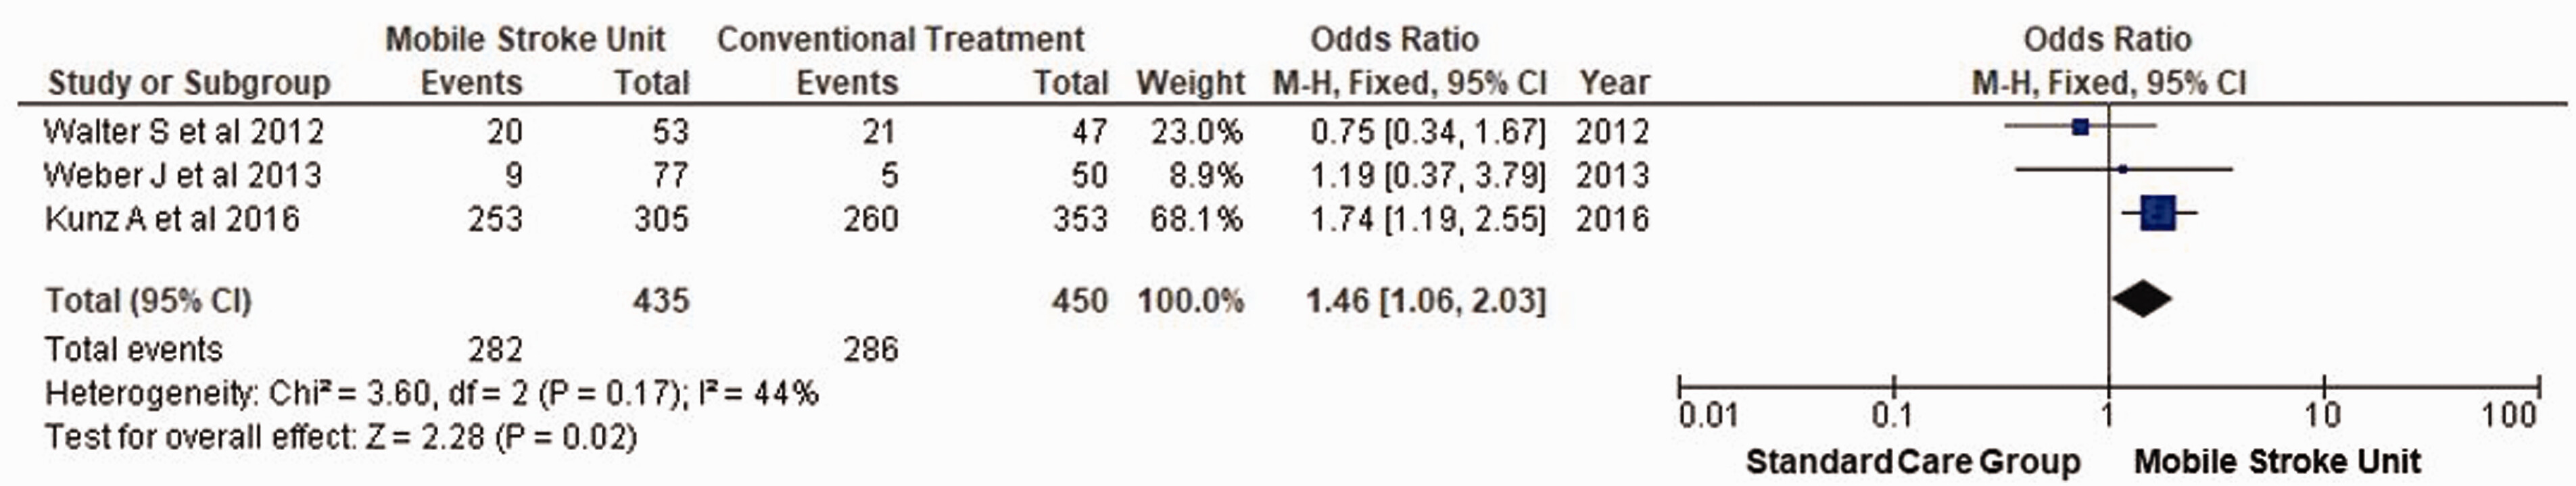
\includegraphics[width=0.5\linewidth]{images_background/fatima_fig_5}
    \caption{Pooled analysis of mRS at 907days (Fatima et al., 2020)}
    \label{fig:background_fatima_fig_5}
\end{figure}


\subsection{Chen review and metanalysis on mobile stroke units 2022 \cite{chen_systematic_2022}}

A total of 22,766 patients from 16 publications were included. In total 7,682 (n = 33.8\%) were treated in the MSU and 15,084 (n = 66.2\%) in the conventional EMS.

Economic analysis were available in four studies, of which two were based on trial data and the others on model simulations. The pooled analysis of time metrics indicated a mean reduction of 33 min and 28 minutes in the time-to-therapy and time-to-CT completion, respectively in the MSU.

There was no significant difference on stroke-related neurological events and in-hospital mortality between the MSU and EMS.

The proportion of patients with modified Ranking scale (mRS) of 0–2 at 90 days from onset was higher in the MSU than EMS (p < 0.05, figure \ref{fig:background_chen_fig_5}). The proportion receiving thrombolysis was 27.7\% in EMS and 37.3\% in MSU. Of those receiving thrombolysis, the proportion mRS0-2 was 59.3\% using EMS and 66.2\% using MSU. In all patients, the proportion mRS0-2 was 58.8\% using EMS and 64.5\% using MSU.

\begin{figure}
    \centering
    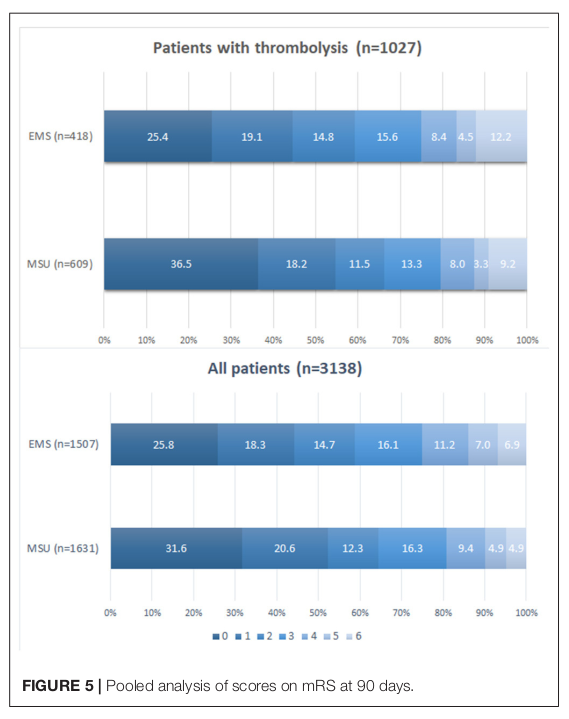
\includegraphics[width=0.9\linewidth]{images_background/chen_fig_5}
    \caption{Pooled analysis of mRS at 90 days (Chen et al., 2021)}
    \label{fig:background_chen_fig_5}
\end{figure}

MSU displayed favorable benefit-cost ratios and incremental cost-effectiveness ratio (\$31,911 /QALY and \$38,731 per DALY) comparing to EMS in multiple economic publications.

Chen et al. did not report on use of thrombectomy;

\subsection{Time to thrombectomy}

The aim of mobile stroke units is often framed as reducing time to thrombolysis  \cite{chen_systematic_2022}, but there is also opportunity to reduce time to thrombectomy, especially by bypass of local IVT-only centre in order to take a patient directly to a MT-capable centre (find ref).

